\begin{center}
\section{Detailed Design Diagram}
\end{center}

\subsection{Data flow Diagrams}
\paragraph{}
A data flow diagram (DFD) is a graphical representation of the "flow" of data through an information system, modelling its process aspects. Often they are a preliminary step used to create an overview of the system which can later be elaborated. DFDs can also be used for the visualization of data processing (structured design).
A DFD shows what kinds of information will be input to and output from the system, where the data will come from and go to, and where the data will be stored. It does not show information about the timing of processes, or information about whether processes will operate in sequence or in parallel (which is shown on a flowchart).
\begin{figure}[h]
\centering
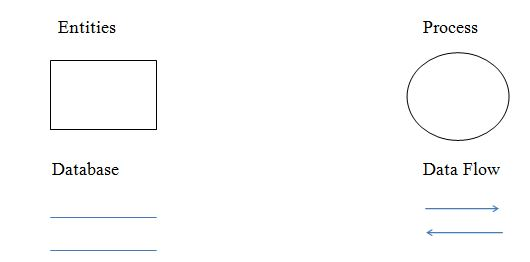
\includegraphics[height=3in, width = 3in]{sym.jpg}
\caption{\emph{Symbols}}
\label{fig:1}
\end{figure}



\paragraph{}
It is common practice to draw the context-level data flow diagram first, which shows the interaction between the system and external agents which act as data sources and data sinks. On the context diagram the system's interactions with the outside world are modelled purely in terms of data flows across the system boundary. The context diagram shows the entire system as a single process, and gives no clues as to its internal organization.
This context-level DFD is next "exploded", to produce a Level 1 DFD that shows some of the detail of the system being modelled. The Level 1 DFD shows how the system is divided into sub-systems (processes), each of which deals with one or more of the data flows to or from an external agent, and which together provide all of the functionality of the system as a whole. It also identifies internal data stores that must be present in order for the system to do its job, and shows the flow of data between the various parts of the system.

\paragraph{}
Data flow diagrams were proposed by Larry Constantine, the original developer of structured design, based on Martin and Estrin's "data flow graph" model of computation.
Data flow diagrams are one of the three essential perspectives of the structured-systems analysis and design method SSADM. The sponsor of a project and the end users will need to be briefed and consulted throughout all stages of a system's evolution. With a data flow diagram, users are able to visualize how the system will operate, what the system will accomplish, and how the system will be implemented. The old system's dataflow diagrams can be drawn up and compared with the new system's data flow diagrams to draw comparisons to implement a more efficient system. Data flow diagrams can be used to provide the end user with a physical idea of where the data they input ultimately has an effect upon the structure of the whole system from order to dispatch to report. How any system is developed can be determined through a data flow diagram model.
In the course of developing a set of levelled data flow diagrams the analyst/designers is forced to address how the system may be decomposed into component sub-systems, and to identify the transaction data in the data model.
\newpage
\begin{figure}[h!]
\centering
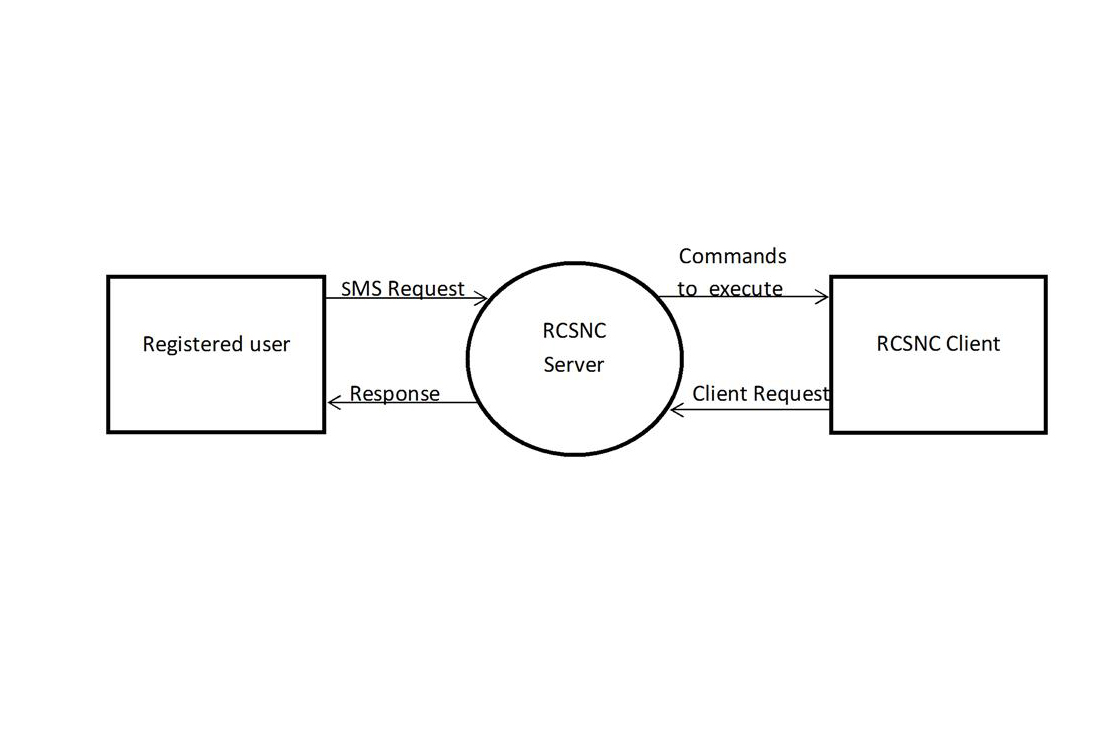
\includegraphics[height=5in, width = 5in]{DFD0.jpg}
\caption{\emph{Level 0 DFD}}
\label{fig:1}
\end{figure}
\newpage
\begin{figure}[h!]
\centering
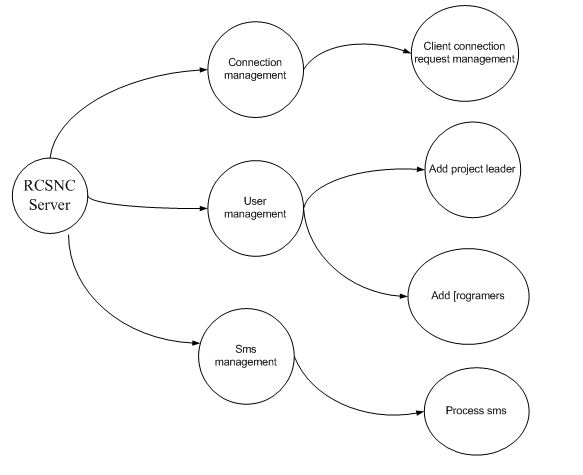
\includegraphics[height=5in, width = 5in]{pic1.jpg}
\caption{\emph{Server Level 1 DFD}}
\label{fig:1}
\end{figure}
\newpage
\begin{figure}[h!]
\centering
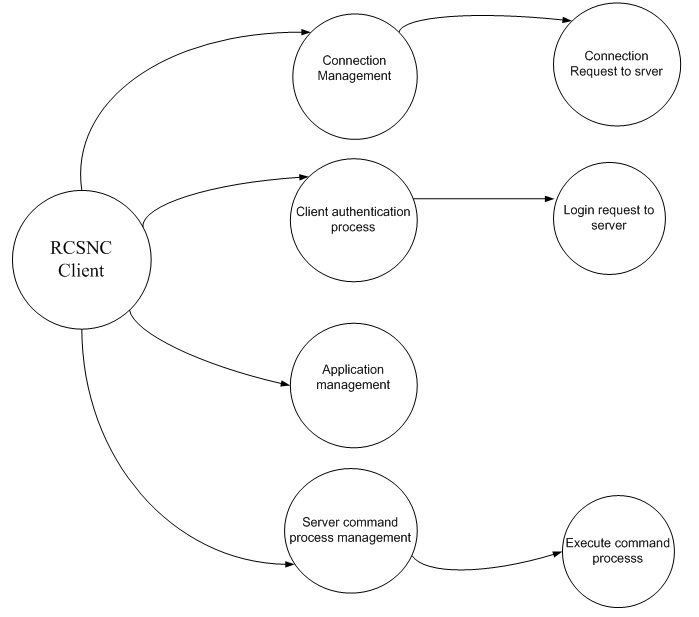
\includegraphics[height=5in, width = 5in]{pict.jpg}
\caption{\emph{Client Level 1 DFD}}
\label{fig:1}
\end{figure}
\newpage
\begin{figure}[h!]
\centering
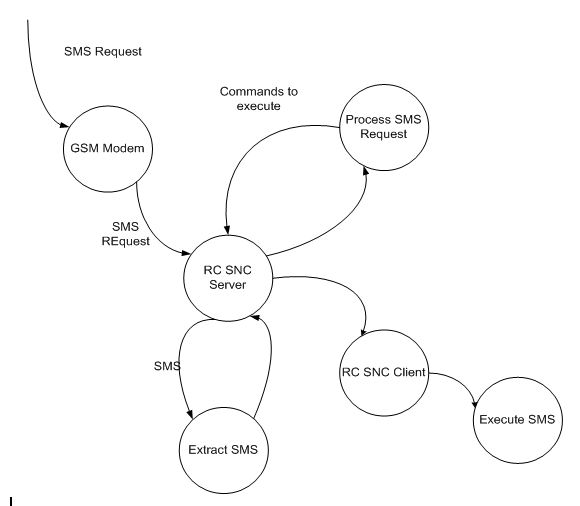
\includegraphics[height=5in, width = 5in]{pic3.jpg}
\caption{\emph{Server Level 2 DFD}}
\label{fig:1}
\end{figure}
\newpage
\begin{figure}[h!]
\centering
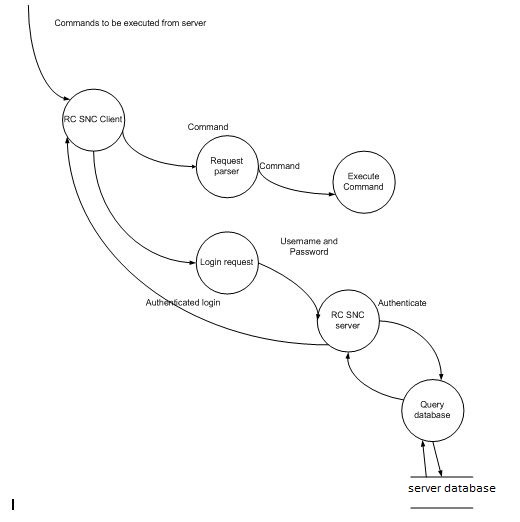
\includegraphics[height=5in, width = 5in]{pic4.jpg}
\caption{\emph{Client Level 2 DFD}}
\label{fig:1}
\end{figure}
\newpage

\subsection{Use case Diagram }
\begin{figure}[h!]
\centering
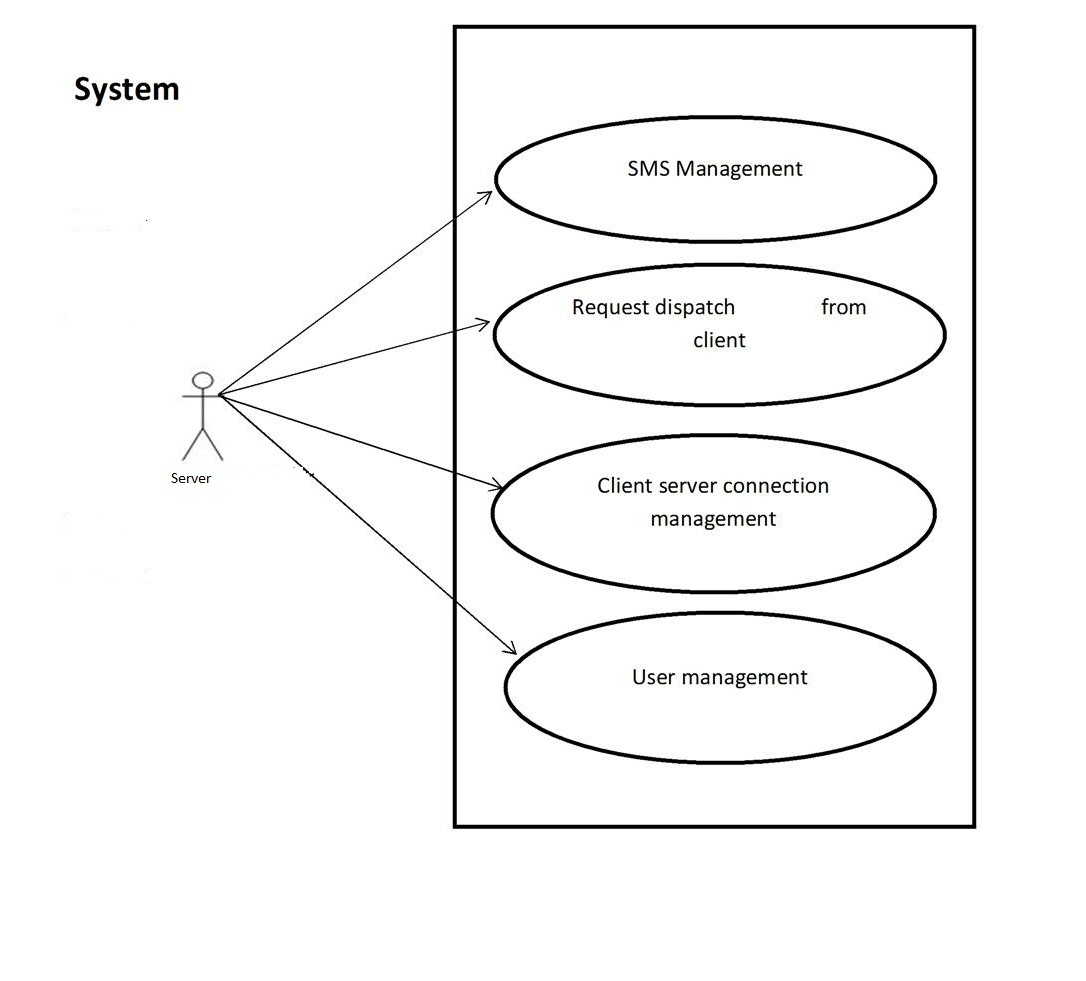
\includegraphics[height=6in, width = 6in]{U2.jpg}
\caption{\emph{Server Usecase Diagram}}
\label{fig:1}
\end{figure}
\newpage
\begin{figure}[h!]
\centering
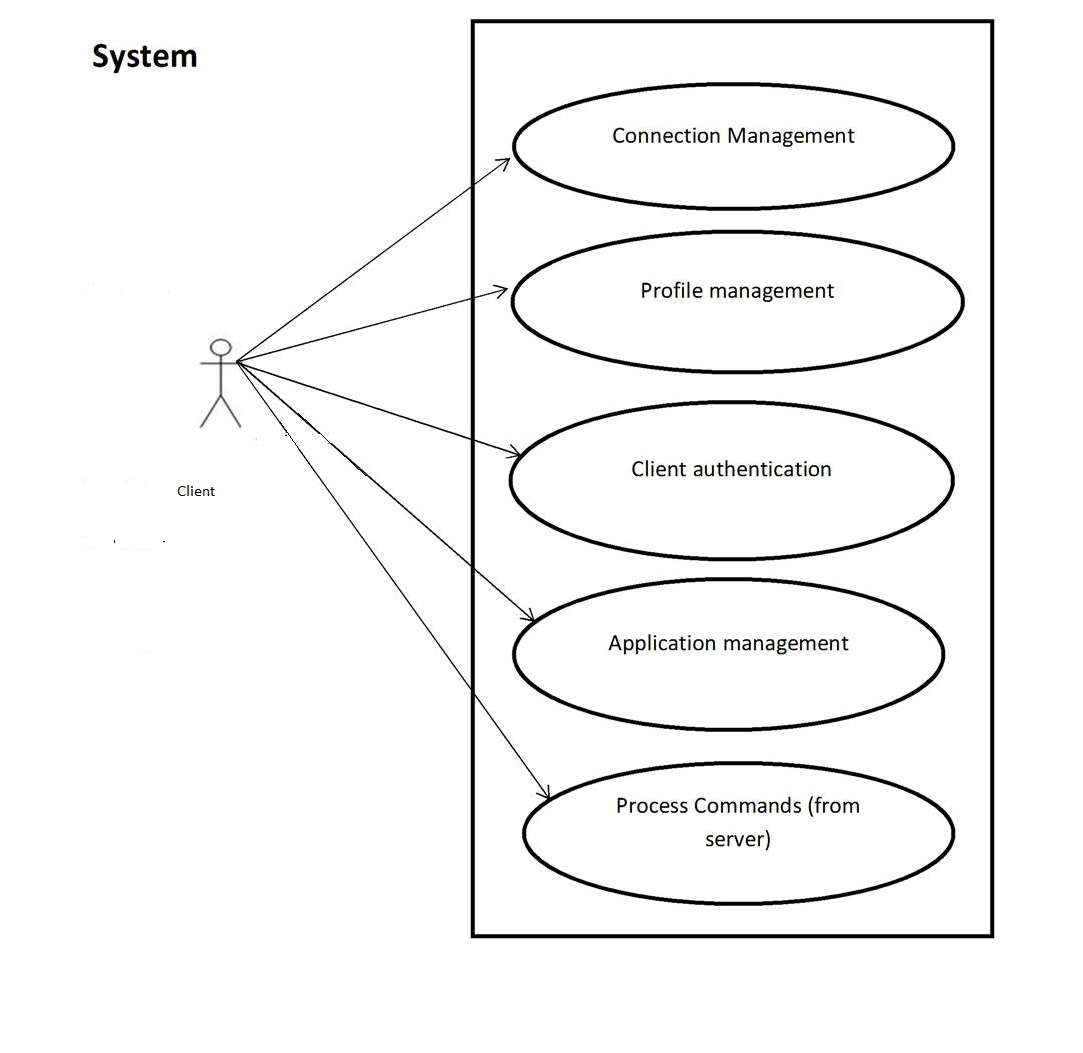
\includegraphics[height=7in, width = 5in]{u.jpg}
\caption{\emph{Client Usecase Diagram}}
\label{fig:1}
\end{figure}


\newpage
\subsection{ Database Table}

\begin{table}[h]
\begin{center}
\begin{large}
\begin{tabular}{|c|c|c|}
\hline 
Field & Data Type & Description \\ 
\hline 
commandId & varchar & primary key \\ 
\hline 
content & varchar & • \\ 
\hline 
mobile & int & • \\ 
\hline 
\end{tabular} 
\textbf{\caption{command}}
\end{large}
\end{center}
\end{table}

\begin{table}[h]
\begin{center}
\begin{large}
\begin{tabular}{|c|c|c|}
\hline 
Field & Data Type & Description\\ 
\hline 
hostId & int & primary key \\ 
\hline 
hardwareInfo & varchar & • \\ 
\hline 
hostName & varchar & • \\ 
\hline 
osinfo & varchar & • \\ 
\hline 
systemInfo & varchar & • \\ 
\hline 
\end{tabular} 
\textbf{\caption{host}}
\end{large}
\end{center}
\end{table}

\begin{table}[h]
\begin{center}
\begin{large}
\begin{tabular}{|c|c|c|}
\hline 
Field & Data Type & Description \\ 
\hline 
leaderId & int & primary key \\ 
\hline 
mobile & int & • \\ 
\hline 
name & varchar & • \\ 
\hline 
\end{tabular} 
\textbf{\caption{leader}}
\end{large}
\end{center}
\end{table}
\newpage

\begin{table}[h]
\begin{center}
\begin{large}
\begin{tabular}{|c|c|c|}
\hline 
Field & Data Type & Description \\ 
\hline 
messageId & int & primary key \\ 
\hline 
message & varchar & • \\ 
\hline 
messageType & int & • \\ 
\hline 
mobile & int & • \\ 
\hline 
\end{tabular} 
\textbf{\caption{message}}
\end{large}
\end{center}
\end{table}

\begin{table}[h]
\begin{center}
\begin{large}

\begin{tabular}{|c|c|c|}
\hline 
Field & Data Type & Description \\ 
\hline 
userId & int & primary key \\ 
\hline 
email & varchar & • \\ 
\hline 
mobile & int & • \\ 
\hline 
name & varchar & • \\ 
\hline 
leaderId & int & • \\ 
\hline 
\end{tabular} 
\textbf{\caption{user}}
\end{large}
\end{center}
\end{table}

